\documentclass[11pt]{article}
 
\usepackage[margin=1in]{geometry} 
\usepackage{amsmath,amsthm,amssymb}
\usepackage[framed,numbered,autolinebreaks,useliterate]{mcode}
\usepackage{graphicx}
\usepackage[ruled,linesnumbered]{algorithm2e}
\usepackage{caption}
\usepackage{subcaption}

\newcommand{\N}{\mathbb{N}}
\newcommand{\Z}{\mathbb{Z}}
 
\newenvironment{theorem}[2][Theorem]{\begin{trivlist}
\item[\hskip \labelsep {\bfseries #1}\hskip \labelsep {\bfseries #2.}]}{\end{trivlist}}
\newenvironment{lemma}[2][Lemma]{\begin{trivlist}
\item[\hskip \labelsep {\bfseries #1}\hskip \labelsep {\bfseries #2.}]}{\end{trivlist}}
\newenvironment{exercise}[2][Exercise]{\begin{trivlist}
\item[\hskip \labelsep {\bfseries #1}\hskip \labelsep {\bfseries #2.}]}{\end{trivlist}}
\newenvironment{problem}[2][Problem]{\begin{trivlist}
\item[\hskip \labelsep {\bfseries #1}\hskip \labelsep {\bfseries #2.}]}{\end{trivlist}}
\newenvironment{question}[2][Question]{\begin{trivlist}
\item[\hskip \labelsep {\bfseries #1}\hskip \labelsep {\bfseries #2.}]}{\end{trivlist}}
\newenvironment{corollary}[2][Corollary]{\begin{trivlist}
\item[\hskip \labelsep {\bfseries #1}\hskip \labelsep {\bfseries #2.}]}{\end{trivlist}}
 
\begin{document}
 
% --------------------------------------------------------------
%                         Start here
% --------------------------------------------------------------
 
\title{ECE 549 Computer Vision: Homework 3}
\author{Xianming Liu} %if necessary, replace with your course title
 
\maketitle
 
\section{Single-View Metrology}

\subsection{Vanishing Points and Vanishing Lines}
After determining the parallel lines in images, the vanishing points could be obtained by using cross product of two parallel lines. In my implementation, I use the criteria that the best Vanishing Points minimizes the angles between itself and center points of all the lines to choose VP. Detailed implementation is in \emph{getVP.m}.
Figure~\ref{fig:vp1}, \ref{fig:vp2} \ref{fig:vp3} show the detected Vanishing points on X, Y, Z directions respecetively.

\begin{figure}[htb]
\begin{center}
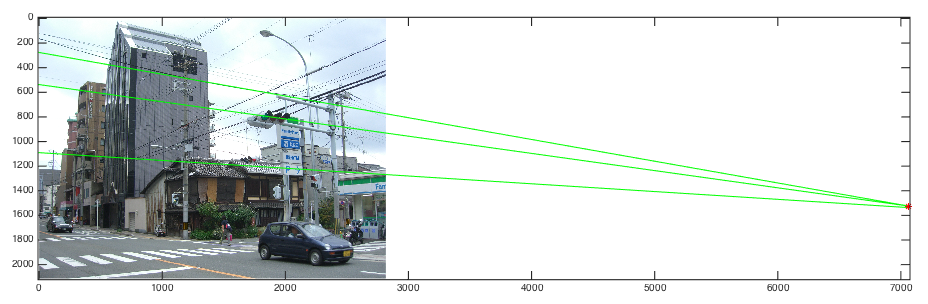
\includegraphics[width=0.9\linewidth]{vp1.png}
\caption{Vanishing Point X: $10^3 * [7.4953, 1.5383, 0.0010]$}
\label{fig:vp1}
\end{center}
\end{figure}

\begin{figure}[htb]
\begin{center}
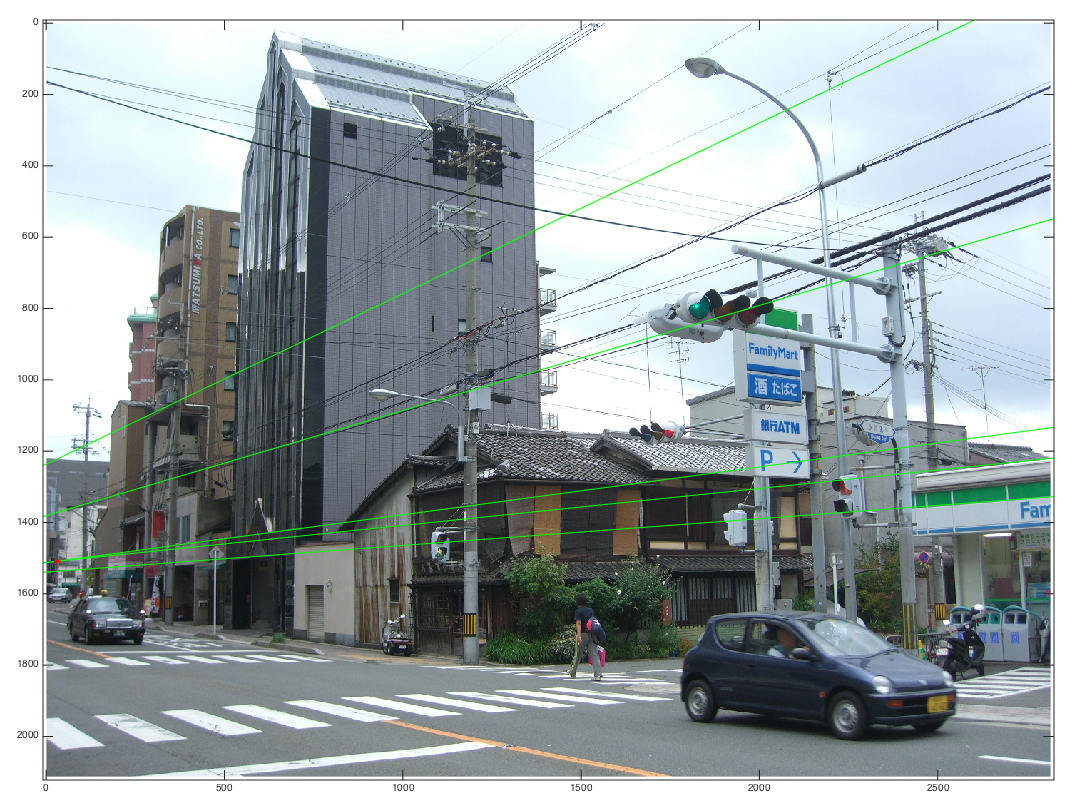
\includegraphics[height=0.4\linewidth]{vp2.png}
\caption{Vanishing Point Y: $10^3 * [0.0304, 1.5086, 0.0010$].}
\label{fig:vp2}
\end{center}
\end{figure}

\begin{figure}[htb]
\begin{center}
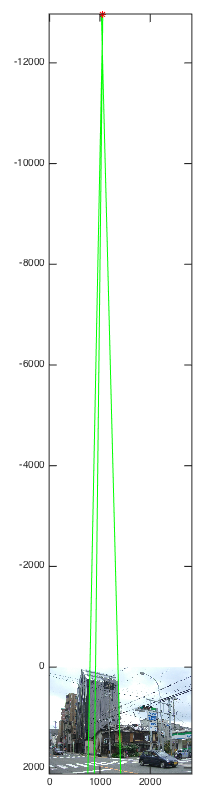
\includegraphics[height=0.5\linewidth]{vp3.png}
\caption{Vanishing Point Z: $10^3 * [1.1216, -6.4439, 0.0010]$}
\label{fig:vp3}
\end{center}
\end{figure}

Horizon vanishing line could be estimated by taking cross product of VP1 and VP2 (both in horizon directions), which is $10^3 * [1.1216, -6.4439, 0.0010]$.

\begin{figure}[htb]
\begin{center}
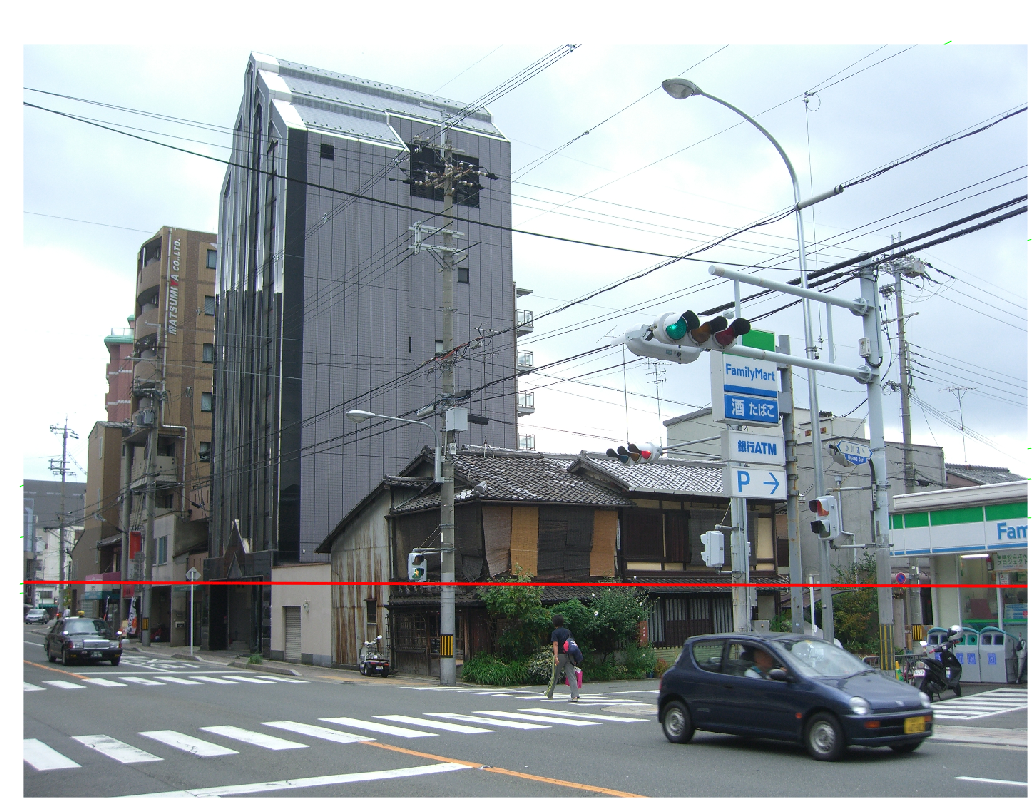
\includegraphics[height=0.6\linewidth]{hvline.png}
\caption{Horizontal Vanishing Line, estimated by two VPs, $1.0e+03 * [0.0000, -0.0010, 1.5185]$.}
\label{fig:hvline}
\end{center}
\end{figure}

\subsection{Focal Length and Optical Center}
Given the intrinsic matrix as 
\[
K = \left( \begin{array}{ccc}
f & 0 & u_0 \\
0 & f & v_0 \\
0 & 0 & 1  \end{array} \right)
\],

and vanishing points $X_i^T X_j = 0$, $\forall i \neq j$, we can use the estimated three vanishing points to estimate the intrinsic matrix $K$, by taking:
\[
X_i^T X_j = p_i^T K^{-T} K^{-1} p_j = 0,\text{} \forall i\neq j
\], 
because the rotation matrix $R^T R = I$. Moreover, 
\[
K^{-T} K^{-1} = \left( \begin{array}{ccc}
1/f^2       &       0       & -u_0/f^2 \\
0           & 1/f^2         & -v_0/f^2 \\
-u_0/f^2    & -v_0/f^2      & \frac{u_0^2+v_0^2}{f^2} + 1  
\end{array} \right)
\]. 

By involving symbol variables in Matlab command \emph{solve}, we can get the solution:
$f = 2248.48$, $(u_0, v_0) = (803.52, 1247.62)$.

\subsection{Rotation Matrix}
Solving the rotation matrix also relies on the detected three vanishing points. Since
\[
\omega \left( \begin{array}{c} u\\v\\1 \end{array} \right) = K R \left( \begin{array}{c} X\\Y\\Z \end{array} \right)
\], 

we use the correspondences between $p_1$ and $[1, 0, 0]$, $p_2$ and $[0, 1, 0]$, $p_3$ and $[0, 0, 1]$ to solve each column of rotation matrix $R$, as:
\[
\omega_1 * p_1 = KR \left( \begin{array}{c} 1\\0\\0 \end{array} \right) = Kr_1
\]
\[
\omega_2 * p_2 = KR \left( \begin{array}{c} 0\\1\\0 \end{array} \right) = Kr_2
\]
\[
\omega_3 * p_3 = KR \left( \begin{array}{c} 0\\0\\1 \end{array} \right) = Kr_3
\]
and the constraints that $R * R^T = I$ to solve rotation matrix $R$, and got:

\[
R = \left( \begin{array}{ccc}
0.9499   & -0.3123   & -0.0119\\
0.0499   & 0.1140    & 0.9922 \\
0.3085   & 0.9431    & -0.1238
\end{array} \right)
\],

\subsection{Height Estimation}
\begin{itemize}
\item[First] Estimate the horizon line: $p_1 = 1.0e+03 * [6.3995, 1.3115, 0.0010]$, $p_2 = 1.0e+03 * [-1.4942, 1.2491, 0.0010]$. And horizon line is got by cross product of $p_1$ and $p_2$: $[0, -0.0008, 1.000]$
\end{itemize}

\bibliographystyle{IEEEbib}
\bibliography{ref}
 
\end{document}
